\section{Experiments}
\label{sec:experiments}

\begin{figure*}[t]
\centering
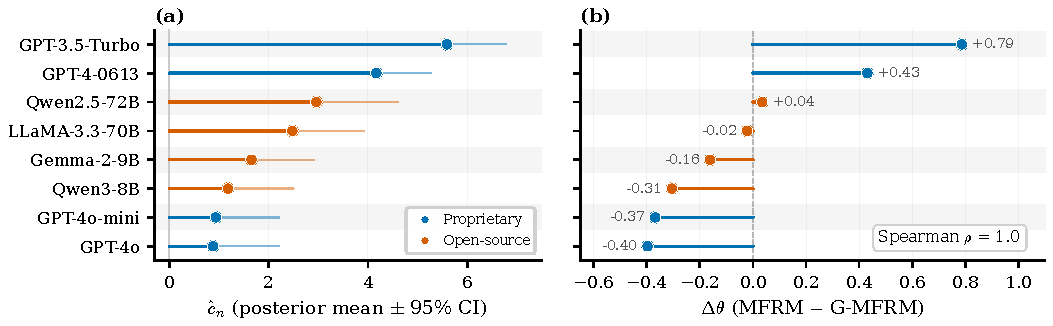
\includegraphics[width=\textwidth]{fig5_6_combined}
\caption{Contamination diagnostics ($N = 8$ pilot, 9 judges). (a)~Contamination susceptibility $\hat{c}_n$ (posterior mean $\pm$ 95\% CI), ordered by magnitude. Older models (GPT-3.5-Turbo, GPT-4-0613) show 4--6$\times$ higher susceptibility than recent models (GPT-4o). (b)~Ability bias absorbed by MFRM-only estimation: $\Delta\theta = \hat{\theta}_{\mathrm{MFRM}} - \hat{\theta}_{\mathrm{G\text{-}MFRM}}$. The monotonic relationship (Spearman $\rho = 1.0$; $N = 8$, interpret with caution) confirms that contamination inflates MFRM ability estimates for high-$c_n$ models, as predicted by the OVB analysis (Section~\ref{sec:confounding}).}
\label{fig:contamination_and_bias}
\end{figure*}

\subsection{Setup}
\label{sec:setup}

Our main experiment uses $N = 17$ target models evaluated by 6 LLM judges; a smaller $N = 8$ pilot with 9 judges validates sample-size effects. Table~\ref{tab:main_results} reports both configurations as part of the coverage analysis.

\paragraph{Data and models.} We evaluate on Arena-Hard \citep{li2024arenahard}, a benchmark of 500 multi-turn conversational items selected for high separability among frontier models. The evaluation uses all 500 items in a connected incomplete design (${\sim}$58\% fill rate of the $N \times I \times J$ tensor). Seventeen target models spanning proprietary and open-source families are evaluated: GPT-4o, GPT-4o-mini, Qwen2.5-72B, LLaMA-3.3-70B, Qwen3-8B, Gemma-2-9B, GPT-4-0613, GPT-3.5-Turbo, Claude-3.5-Sonnet, GPT-4-Turbo, LLaMA-3.1-70B, Gemma-2-27B, Claude-3-Opus, LLaMA-3-70B, Mixtral-8x22B, Claude-3-Haiku, and LLaMA-3-8B. Ground-truth rankings are derived from Chatbot Arena human preference data \citep{zheng2023mtbench}.

\paragraph{Judges.} Six LLM judges score responses in position-swapped pairwise mode: Claude Sonnet 4.6, DeepSeek-V4-Pro, Gemini-2.5-Pro, LLaMA-3.3-70B, Qwen2.5-72B, and Qwen3-235B. Four provide complete item coverage; two (Gemini, Sonnet) cover ${\sim}$60--79\% of items; this yields an incomplete connected design. Two models serve as both judge and target; $d_j$ absorbs self-evaluation bias ($\tau$ unchanged when excluding self-judging; Appendix~\ref{app:self_eval}).

\paragraph{Exposure estimation.} Per-item $e_i$ follows the two-source pipeline in \S\ref{sec:staged} (75\% reference anchoring, 25\% cross-model agreement; robust to weight configuration, $\rho \geq 0.998$; Appendix~\ref{app:weight_robustness}).

\paragraph{MCMC.} NumPyro \citep{phan2019numpyro} NUTS, 6{,}000 warmup $+$ 4{,}000 samples $\times$ 4 chains (target acceptance 0.95). Convergence: $\hat{R} < 1.05$, ESS $> 100$ \citep{vehtari2021rhat, gelman2013bda}.

\subsection{Main Results}
\label{sec:main_results}

\begin{table}[t]
\centering
\footnotesize
\setlength{\tabcolsep}{3.5pt}
\begin{tabular}{lccccc}
\toprule
\textbf{Item Set} & \textbf{Items} & \textbf{Cov.} & $\tau_{\mathrm{raw}}$ & $\tau_{\mathrm{G\text{-}MFRM}}$ & $\Delta\tau$ \\
\midrule
\multicolumn{6}{l}{\textit{$N = 17$, 6 judges (main experiment)}} \\
Full set & 500 & 46\% & 0.838 & 0.794 & $-$0.044 \\
Filtered & 317 & 73\% & 0.824 & 0.809 & $-$0.015 \\
Exposed-only & 231 & 100\% & 0.779 & 0.779 & \phantom{$-$}0.000 \\
\midrule
\multicolumn{6}{l}{\textit{$N = 8$, 9 judges (pilot)}} \\
Full set & 176 & -- & 0.786 & 0.857$^{\dagger}$ & $+$0.071 \\
\bottomrule
\end{tabular}
\caption{Ranking accuracy (Kendall $\tau$ against Chatbot Arena) as a function of exposure coverage. G-MFRM over-correction decreases across all three coverage levels ($\Delta\tau$: $-0.044 \to -0.015 \to 0.000$). At full coverage, G-MFRM matches the raw average exactly; the pilot ($N = 8$) suggests positive $\Delta\tau$ when coverage is adequate. All seven baselines (MFRM-only, Sequential, CyclicJudge, DCR Factor, Pref.\ Leakage) produce $\tau$ within 0.015 of the raw average at both panel sizes. $^{\dagger}$Bootstrap $\Delta\tau$ CI includes zero.}
\label{tab:main_results}
\end{table}

We compare G-MFRM against seven baselines that address judge bias or contamination separately (Table~\ref{tab:main_results}): Raw Average, MFRM-only (Eq.~\ref{eq:mfrm}), Sequential (MFRM then contamination adjustment), CyclicJudge \citep{cyclicjudge2026}, CyclicJudge+discard, DCR Factor \citep{dcr2025}, and Preference Leakage calibration \citep{preference_leakage2026}. All methods are evaluated by Kendall $\tau$ and Spearman $\rho$ against Chatbot Arena human rankings.

\paragraph{Synthetic validation.} On synthetic data ($N = 50$, 20 seeds), G-MFRM reduces ability RMSE by 51\% relative to sequential estimation ($p < 10^{-5}$) and improves ranking accuracy ($\tau$: $0.922$ vs.\ $0.839$, Wilcoxon $p < 0.001$). Contamination susceptibility is recovered with Pearson $r = 0.81$.

\paragraph{Predictive fit.} In the $N = 8$ pilot, Leave-one-out (LOO) cross-validation strongly favors G-MFRM over MFRM-only (Expected Log Pointwise Predictive Density difference $\Delta\mathrm{ELPD}_{\mathrm{LOO}} = -55.7$, SE $= 9.4$, $|\Delta/\mathrm{SE}| = 5.9$; \citealp{vehtari2017loo}), with stacking weight 1.0 and all Pareto $\hat{k} < 0.7$ (Appendix~\ref{app:loo_comparison}).

\paragraph{Reconciling predictive fit and ranking accuracy.} The LOO improvement and the ranking degradation are not contradictory: they measure different quantities. LOO-ELPD evaluates observation-level predictive accuracy across all $(n, i, j)$ triples: it rewards the model for capturing contamination structure in individual responses. Kendall $\tau$ evaluates aggregate system-level rankings, which are sensitive to the accuracy of per-item exposure estimates $e_i$. The separation indicates that the contamination signal is real (the model fits better), but incomplete exposure coverage causes the correction to over-correct when aggregated to rankings. The coverage ablation below confirms this interpretation.

\paragraph{Exposure coverage and ranking accuracy.} G-MFRM's ranking accuracy on real data depends on exposure estimation quality. At $N = 17$, the full item set (500 items) has only 46\% of items with non-zero exposure estimates; G-MFRM over-corrects on the remaining items, and the result is $\Delta\tau = -0.044$ relative to the raw average ($\tau = 0.794$ vs.\ $0.838$). We trace this degradation through three item subsets with increasing exposure coverage:
%
\begin{itemize}
    \item Full set (500 items, 46\% $e_i > 0$): $\Delta\tau = -0.044$
    \item Filtered set (317 items, 73\% $e_i > 0$): $\Delta\tau = -0.015$
    \item Exposed-only (231 items, 100\% $e_i > 0$): $\Delta\tau = 0.000$
\end{itemize}
%
This controlled ablation ($-0.044 \to -0.015 \to 0.000$) demonstrates that over-correction is attributable to incomplete exposure coverage. Two additional variants confirm the mechanism: MFRM-only on the filtered set yields $\Delta\tau = 0.000$, which isolates the degradation to the contamination gating term; a contamination-only variant without severity modeling yields $\Delta\tau = -0.118$, evidence that naive linear contamination deduction without joint calibration is catastrophically harmful.

\paragraph{Contamination diagnostics.} G-MFRM's primary real-data contribution is interpretable per-model contamination estimation. In the $N = 8$ pilot, the contamination susceptibility profile (Figure~\ref{fig:contamination_and_bias}a) reveals a clear gradient by model age: older models show $\hat{c}_n > 4$ (GPT-3.5-Turbo: $5.60$; GPT-4-0613: $4.20$), while recent models show near-zero susceptibility (GPT-4o: $0.88$; GPT-4o-mini: $0.93$). MFRM-only estimation absorbs this contamination signal into ability estimates, inflating $\hat{\theta}$ for the most contaminated models by up to 0.79 logits (Figure~\ref{fig:contamination_and_bias}b; Spearman $\rho = 1.0$ between $\hat{c}_n$ and $\Delta\theta$, though with only $N = 8$ data points, perfect rank correlation is not statistically remarkable and should not be interpreted as a robust finding). The $N = 17$ analysis preserves the same age gradient at lower absolute scale (GPT-3.5-Turbo: $2.57$; GPT-4-0613: $3.78$), consistent with shrinkage from the larger model population. All parameters achieve $\hat{R} \leq 1.003$ with ESS $\geq 1{,}240$ in the $N = 17$ analysis (Appendices~\ref{app:item_diagnostics} and~\ref{app:ppc}).

\paragraph{Judge severity and panel design.} Judge severity profiles vary across the panel (Figure~\ref{fig:judge_severity}), and contamination--ability separation improves with severity diversity: panels with $k \geq 4$ judges covering the severity extremes provide the most reliable diagnostic output (Appendix~\ref{app:judge_count}). Leave-one-judge-out analysis identifies three individually necessary judges---those at the strict and lenient extremes of the $d_j$ distribution---whose removal reduces G-MFRM $\tau$ to the baseline. This finding suggests that judge panels should prioritize scoring tendency diversity over judge count alone.


\subsection{Error Propagation and Ablation}
\label{sec:error_prop_results}

\begin{figure}[t]
\centering
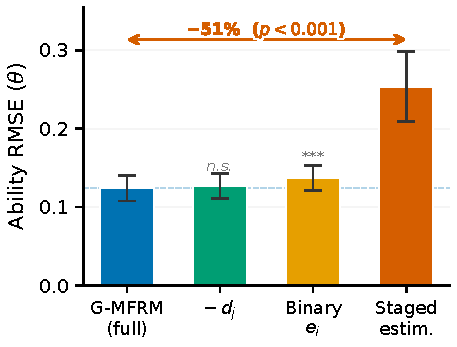
\includegraphics[width=\columnwidth]{fig_ablation_rmse}
\caption{Ablation on synthetic data ($N = 50$, 20 seeds). Joint estimation drives the improvement: staged estimation doubles $\theta$-RMSE ($p < 0.001$). Continuous gating provides a moderate gain over binary ($p < 0.001$); removing judge severity $d_j$ has negligible effect on ability recovery (n.s.).}
\label{fig:ablation}
\end{figure}

Table~\ref{tab:error_prop} validates the theoretical prediction (\S\ref{sec:error_prop}): below $\sigma = 0.2$, ability RMSE increases by 5.9\% and contamination RMSE by 7.9\%; beyond the threshold ($\sigma = 0.5$), degradation becomes substantial. Ablation (Figure~\ref{fig:ablation}; full results in Table~\ref{tab:ablation}, Appendix~\ref{app:ablation}) confirms joint estimation as the dominant contributor ($2.0\times$ $\theta$-RMSE increase under staged estimation, $p < 0.001$) and continuous gating over binary ($c_n$-RMSE $-$40\%, $p < 0.001$).